% !TEX root = saveliev_physics_general_course_2.tex
%!TEX TS-program = pdflatex
%!TEX encoding = UTF-8 Unicode
\chapter[Năng lượng điện trường]{Năng lượng \\điện trường}\label{chap:4}
\chaptermark{Năng lượng điện trường}

\section{Năng lượng của vật dẫn tích điện}\label{sec:4_1}

Điện tích $q$ trên một vật dẫn có thể được xem là một hệ các điện tích điểm $\Delta{q}$. Trong \sect{1_7}, ta thu được biểu thức sau cho năng lượng tương tác của một hệ các điện tích [xem \eqn{1_39}]:
\begin{equation}\label{eq:4_1}
	\ab{W}{p} = \frac{1}{2} \sum_i q_i \varphi_i.
\end{equation}

\noindent
Ở đây, $\varphi_i$ là điện thế gây ra bởi các điện tích khác ngoài $q_i$ tại vị trí đặt $q_i$.

Bề mặt vật dẫn là đẳng thế. Do đó, điện thế tại vị trí của các điện tích điểm $\Delta{q}$ là bằng nhau và bằng điện thế $\varphi$ của vật dẫn. Sử dụng \eqn{4_1}, ta thu được phương trình mô tả năng lượng của một vật dẫn tích điện

\begin{equation}\label{eq:4_2}
	\ab{W}{p} = \frac{1}{2} \sum \varphi \Delta{q} = \frac{1}{2} \varphi \sum \Delta{q} = \frac{1}{2} \varphi q.
\end{equation}

\noindent
Xét thêm \eqn{3_5}, ta có thể viết thành
\begin{equation}\label{eq:4_3}
	\ab{W}{p} = \frac{\varphi q}{2} = \frac{q^2}{2 C} = \frac{C \varphi^2}{2}.
\end{equation}

\noindent
Bất kỳ biểu thức nào trong số chúng đều cho biết năng lượng của một vật dẫn tích điện.

\section{Năng lượng của tụ điện}\label{sec:4_2}

Xem rằng điện thế của bản tụ phẳng mang điện tích $+q$ là $\varphi_1$, của bản còn lại mang điện tích $-q$ là $\varphi_2$. Do đó, mỗi điện tích cơ bản $\Delta{q}$ được chia nhỏ ra từ $+q$ đều ở điểm có điện thế bằng $\varphi_1$, và mỗi điện tích được chia nhỏ ra từ $-q$ đều ở điểm có điện thế bằng $\varphi_2$. Từ \eqn{4_1}, năng lượng của một hệ điện tích như vậy là
\begin{equation}\label{eq:4_4}
	\ab{W}{p} = \frac{1}{2} \bracket{ (+q) \varphi_1 + (-q) \varphi_2} = \frac{1}{2} q \parenthesis{\varphi_1 - \varphi_2} = \frac{1}{2} q U.
\end{equation}

\noindent
Sử dụng \eqn{3_11}, ta có thể viết ba công thức tính năng lượng của vật dẫn tích điện:
\begin{equation}\label{eq:4_5}
	\ab{W}{p} = \frac{q U}{2} = \frac{q^2}{2 C} = \frac{C U^2}{2}.
\end{equation}

\noindent
Phương trình \eqref{eq:4_5} chỉ khác với \eqref{eq:4_3} ở chỗ là chứa $U$ thay vì $\varphi$.

\begin{figure}[!htb]
	\begin{center}
		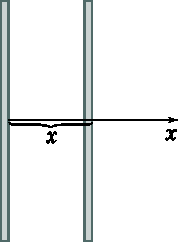
\includegraphics[scale=1]{figures/ch_04/fig_4_1.pdf}
		\caption[]{}
		\label{fig:4_1}
	\end{center}
	\vspace{-0.8cm}
\end{figure}

Biểu thức thế năng cho phép chúng ta tìm lực mà các bản song song của một tụ điện hút lẫn nhau. Chúng ta hãy giả sử rằng khoảng cách giữa các bản có thể thay đổi. Ta có thể gắn gốc tọa độ của trục $x$ với bản bên trái (\fig{4_1}). Từ đó, tọa độ $x$ của bản tụ thứ hai sẽ xác định khoảng cách giữa hai tấm bản. Dựa vào \eqns{3_12}{4_5}, ta có
%The expression for the potential energy permits us to find the force with which the plates of a parallel-plate capacitor attract each other. Let us assume that the separation distance of the plates can be changed. We shall associate the origin of the $x$-axis with the left-hand plate (\fig{4_1}). The coordinate $x$ of the second plate will, therefore, determine the separation distanced of the plates. According to \eqns{3_12}{4_5}, we have
\begin{equation*}
	\ab{W}{p} = \frac{q^2}{2 C} = \frac{q^2}{2 \varepsilon_0 \varepsilon S} x.
\end{equation*}

\noindent
Hãy đạo hàm biểu thức này theo biến x, giả sử rằng điện tích của hai bản là không đổi (tụ điện đã được ngắt khỏi nguồn điện). Kết quả là ta được thành phần theo phương $x$ của lực tác dụng lên bản bên phải:
\begin{equation*}
	F_x = - \diffpartial{\ab{W}{p}}{x} = - \frac{q^2}{2 \varepsilon_0 \varepsilon S}.
\end{equation*}

\noindent
Độ lớn của biểu thức này cho biết lực mà các bản hút nhau:
\begin{equation}\label{eq:4_6}
	F = \frac{q^2}{2 \varepsilon_0 \varepsilon S}.
\end{equation}

Bây giờ, hãy tính lực hút giữa hai bản tụ song song bằng tích của điện trường do một bản tạo ra và điện tích tập trung trên bản còn lại. Bằng \eqn{1_120}, độ lớn của điện trường do một bản tạo ra là 
\begin{equation}\label{eq:4_7}
	E = \frac{\sigma}{2 \varepsilon_0} = \frac{q}{2 \varepsilon_0 S}.
\end{equation}

\noindent
Một chất điện môi làm suy yếu điện trường trong vùng không gian giữa các bản đi $e$ lần, nhưng điều này chỉ xảy ra bên trong chất điện môi [xem \eqn{2_33} và các nội dung liên quan]. Các điện tích trên bản tụ nằm ngoài lớp điện môi, do đó chịu tác dụng của cường độ điện trường trong \eqn{4_7}. Nhân điện tích của một tấm $q$ với cường độ này, chúng ta có biểu thức sau cho lực:
% A dielectric weakens the field in the space between the plates $e$ times, but this occurs only inside the dielectric [see \eqn{2_33} and the related text]. The charges on the plates are outside the dielectric and are, therefore, acted upon by the field strength given by \eqn{4_7}. Multiplying the charge of a plate $q$ by this strength, we get the following expression for the force:
\begin{equation}\label{eq:4_8}
	F' = \frac{q^2}{2 \varepsilon_0 S}.
\end{equation}

Hai phương trình \eqref{eq:4_6} và \eqref{eq:4_8} không tương đồng.  Độ lớn của lực cho bởi \eqn{4_6} thu được từ biểu thức cho năng lượng phù hợp với dữ liệu thực nghiệm. Ta giải thích như sau: ngoài lực ``điện'' trong \eqn{4_8}, các bản còn chịu tác dụng của các lực cơ học từ chất điện môi có xu hướng tách chúng ra xa nhau (xem \sect{2_8}; chúng ta phải lưu ý rằng chúng ta nghĩ đến một chất điện môi lỏng). Có một điện trường phân tán ở rìa của các bản, điện trường này có cường độ giảm dần khi khoảng cách đến rìa bản tăng (\fig{4_2}). Các phân tử của chất điện môi có moment lưỡng cực và chịu tác dụng của một lực kéo chúng vào vùng có điện trường mạnh hơn [xem \eqn{1_62}]. Kết quả là áp suất giữa các bản tăng lên và xuất hiện một lực làm yếu đi lực cho bởi \eqn{4_8} $e$ lần.
%The value of the force given by \eqn{4_6} obtained from the expression for the energy agrees with experimental data. The explanation is that apart from the ``electric'' force given by \eqn{4_8}, the plates experience mechanical forces from the side of the dielectric that tend to spread them apart (see \sect{2_8}; we must note that we have in mind a fluid dielectric). There is a dispersed field at the edges of the plates whose magnitude diminishes with an increasing distance from the edges (\fig{4_2}). The molecules of the dielectric have a dipole moment and experience the action of a force pulling them into the region with the stronger field [see \eqn{1_62}]. The result is an increase in the pressure between the plates and the appearance of a force that weakens the force given by \eqn{4_8} $e$ times.

\begin{figure}[!htb]
	\begin{minipage}[t]{0.48\linewidth}
		\begin{center}
			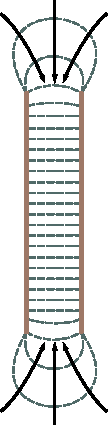
\includegraphics[scale=1]{figures/ch_04/fig_4_2.pdf}
			\caption[]{}
			\label{fig:4_2}
		\end{center}
	\end{minipage}
	\hfill{ }%space{-0.05cm}
	\begin{minipage}[t]{0.48\linewidth}
		\begin{center}
			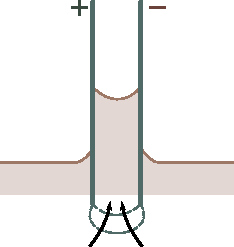
\includegraphics[scale=1]{figures/ch_04/fig_4_3.pdf}
			\caption[]{}
			\label{fig:4_3}
		\end{center}
	\end{minipage}
\vspace{-0.4cm}
\end{figure}

Nếu một tụ điện không khí được tích điện và được nhúng một phần vào chất điện môi lỏng thì chất lỏng sẽ bị hút vào khoảng không giữa các bản (\fig{4_3}). Hiện tượng này được giải thích như sau. Hằng số điện môi của không khí gần như bằng một. Do đó, trước khi các bản được nhúng vào chất điện môi, ta có thể xem rằng điện dung của tụ điện là $C_0=\varepsilon_0S/d$ và năng lượng của nó là $W_0=q^2/2C_0$. Khi không gian giữa các bản được lấp đầy một phần bằng chất điện môi, tụ có thể được coi là hai tụ điện được mắc song song, một tụ có diện tích bản tụ là $xS$ ($x$ là tỉ số diện tích của phần được lấp đầy bởi chất lỏng so với điện tích cả bản) chứa đầy chất điện môi có $\varepsilon>1$, và một tụ có diện tích bản tụ bằng $(1-x)S$. Khi được mắc song song, điện dung của chúng được tính tổng: 
%If a charged capacitor with an air gap is partially immersed in a liquid dielectric, the latter will be drawn into the space between the plates (\fig{4_3}). This phenomenon is explained as follows. The permittivity of air virtually equals unity. Consequently, before the plates are immersed in the dielectric, we can consider that the capacitance of the capacitor is $C_0=\varepsilon_0S/d$, and its energy is $W_0=q^2/2C_0$. When the space between the plates is partially filled with the dielectric, the capacitor can be considered as two capacitors connected in parallel, one of which has a plate area of $xS$ ($x$ is the relative part of the space filled with the liquid) and is filled with a dielectric for which $\varepsilon>1$, and the other has a plate area equal to $(1-x)S$. In the parallel connection of capacitors, their capacitances are summated:
\begin{equation*}
	C = C_1 + C_2 = \frac{\varepsilon_0 S (1-x)}{d} + \frac{\varepsilon_0 \varepsilon S x}{d} = C_0 + \frac{\varepsilon_0 (\varepsilon - 1) S}{d} x > C_0.
\end{equation*}

\noindent
Vì $C>C_0$, năng lượng $W=q^2/2C$ sẽ nhỏ hơn $W_0$ (điện tích $q$ xem như không đổi---tụ điện đã được ngắt khỏi nguồn điện trước khi được nhúng trong chất lỏng). Vì vậy, việc lấp đầy không gian giữa các tấm bằng chất điện môi có lợi về mặt năng lượng. Đây là lý do tại sao chất điện môi bị hút vào trong tụ điện và mực chất lỏng dâng lên trong vùng không gian ngăn cách giữa hai bản tụ. Điều này dẫn đến sự gia tăng thế năng hấp dẫn. Về lâu dài, mức điện môi trong không gian sẽ tự xác lập ở một độ cao nhất định, tương ứng với năng lượng tổng cộng (điện và hấp dẫn) nhỏ nhất. Hiện tượng trên tương tự như sự dâng lên mao dẫn của chất lỏng trong khoảng hẹp giữa các bản (xem mục 14.5 của Tập I).

Việc hút chất điện môi vào không gian giữa các bản cũng có thể được giải thích theo quan điểm vi mô. Có một điện trường không đều ở rìa của các bản tụ điện. Các phân tử của chất điện môi có moment lưỡng cực bên trong hoặc thu được dưới tác dụng của điện trường; nên chúng chịu tác dụng của các lực có xu hướng dịch chuyển chúng sang vùng có điện trường mạnh hơn, tức là vào trong tụ điện. Các lực này làm cho chất lỏng bị hút vào không gian giữa các bản tụ cho đến khi các lực điện tác dụng lên chất lỏng ở phần rìa các bản cân bằng với trọng lượng của cột chất lỏng. 

\section{Năng lượng điện trường}\label{sec:4_3}

Năng lượng của một tụ tích điện có thể được biểu diễn thông qua các đại lượng đặc trưng cho điện trường trong vùng không gian giữa các bản. Hãy làm điều này đối với một tụ điện phẳng (tụ điện có hai bản song song). Đưa biểu thức \eqref{eq:3_12} cho điện dung vào phương trình $\ab{W}{p}=CU^2/2$ [xem \eqn{4_5}], ta được
\begin{equation*}
	\ab{W}{p} = \frac{C U^2}{2} = \frac{\varepsilon_0 \varepsilon S U^2}{2 d} = \frac{\varepsilon_0 \varepsilon}{2} \parenthesis{\frac{U}{d}}^2 S d.
\end{equation*}

\noindent
Tỉ số $U/d$ bằng cường độ điện trường giữa các bản; tích số $Sd$ là thể tích bị điện trường chiếm chỗ. Do đó,
\begin{equation}\label{eq:4_9}
	\ab{W}{p} = \frac{\varepsilon_0 \varepsilon E^2}{2} V.
\end{equation}

Phương trình $\ab{W}{p}=q^2/(2C)$ liên hệ năng lượng của một tụ điện với điện tích trên các bản của nó, trong khi \eqn{4_9} liên hệ năng lượng này với cường độ điện trường. Thật hợp lý khi đặt câu hỏi rằng: rốt cuộc thì năng lượng được dự trữ ở đâu (tức là tập trung ở đâu), vật mang năng lượng là gì---điện tích hay điện trường? Câu hỏi này không thể được trả lời trong phạm vi tĩnh điện học, ngành nghiên cứu các trường của điện tích cố định, không đổi theo thời gian. Các trường không đổi và các điện tích tạo ra chúng không thể tồn tại tách biệt với nhau. Tuy nhiên, các trường biến thiên theo thời gian có thể tồn tại độc lập với các điện tích tạo ra chúng và lan truyền trong không gian dưới dạng sóng điện từ. Thực nghiệm chứng tỏ rằng sóng điện từ truyền tải năng lượng. Cụ thể, năng lượng duy trì sự sống trên Trái Đất được cung cấp từ Mặt trời bằng sóng điện từ; năng lượng làm cho máy thu thanh phát ra âm thanh được mang từ trạm phát bằng sóng điện từ,... Những sự thật này khiến chúng ta nhận ra vật mang năng lượng là một trường. 

Nếu một trường là thuần nhất (đó là trường hợp của tụ điện phẳng), năng lượng giới hạn bên trong nó phân bố trong không gian với mật độ không đổi $w$ bằng năng lượng điện trường chia cho thể tích mà nó chiếm chỗ. Kiểm tra \eqn{4_9} cho thấy mật độ năng lượng của trường có cường độ $E$ được thiết lập trong môi trường có hằng số điện môi $\varepsilon$ là
\begin{equation}\label{eq:4_10}
	w = \frac{\varepsilon_0 \varepsilon E^2}{2}.
\end{equation}

\noindent
Kết hợp với \eqn{2_21}, ta có thể viết \eqn{4_10} như sau:
\begin{equation}\label{eq:4_11}
	w = \frac{\varepsilon_0 \varepsilon E^2}{2} = \frac{E D}{2} = \frac{D^2}{2 \varepsilon_0 \varepsilon}.
\end{equation}

Trong một điện môi đẳng hướng, hướng của các vectơ $\vec{E}$ và $\vec{D}$ trùng nhau. Do đó, chúng ta có thể viết phương trình cho mật độ năng lượng ở dạng
\begin{equation*}
	w = \frac{\vecdot{E}{D}}{2}.
\end{equation*}

\noindent
Thay $\vec{D}$ trong phương trình này bằng giá trị của nó trong \eqn{2_18}, ta nhận được biểu thức sau cho $w$:
\begin{equation}\label{eq:4_12}
	w = \frac{\vec{E} (\varepsilon_0 \vec{E} + \vec{P})}{2} = \frac{\varepsilon_0 \vec{E}^2}{2} + \frac{\vecdot{E}{P}}{2}.
\end{equation}

\noindent
Số hạng đầu tiên của phương trình chính là mật độ năng lượng của trường $\vec{E}$ trong chân không. Số hạng thứ hai, như chúng ta sẽ tiến hành chứng minh, là năng lượng tiêu hao cho sự phân cực của chất điện môi.

Một chất điện môi bị phân cực khi các điện tích chứa trong các phân tử bị dịch chuyển khỏi vị trí của chúng dưới tác dụng của điện trường $\vec{E}$. Công thực hiện để dịch chuyển các điện tích $q$, đi một khoảng $\deriv{\vec{r}_i}$ trên một đơn vị thể tích của chất điện môi là
\begin{equation*}
	\deriv{A} = \sum_{V=i} q_i \vec{E}\, \deriv{\vec{r}_i} = \vec{E}\, \deriv\parenthesis{\sum_{V=i} q_i \vec{r}_i}
\end{equation*}

\noindent
(để cho đơn giản, ta xem điện trường là thuần nhất). Dựa vào \eqn{2_1}, $\sum_{V=i}q_i\vec{r}_i$ bằng moment lưỡng cực của một đơn vị thể tích, tức là, độ phân cực của chất điện môi $\vec{P}$. Vì thế,
\begin{equation}\label{eq:4_13}
	\deriv{A} = \vec{E}\, \deriv{\vec{P}}.
\end{equation}

\noindent
Vector $\vec{P}$ liên hệ với vector $\vec{E}$ bằng biểu thức $\vec{P}=\chi \varepsilon_0\vec{E}$ [xem \eqn{2_5}]. Vì vậy, $\deriv{\vec{P}}=\chi\varepsilon_0\, \deriv{\vec{E}}$. Dử dụng giá trị của $\deriv{\vec{P}}$ trong \eqn{4_13}, ta được biểu thức
\begin{equation*}
	\deriv{A} = \chi \varepsilon_0 \vec{E}\, \deriv{\vec{E}} = \deriv{\parenthesis{\frac{\chi \varepsilon_0 \vec{E}^2}{2}}} = \deriv{\parenthesis{\frac{\vecdot{E}{P}}{2}}}.
\end{equation*}

\noindent
Cuối cùng, tích phân cho chúng ta biểu thức sau tính công cần thực hiện để phân cực một đơn vị thể tích của chất điện môi:
\begin{equation}\label{eq:4_14}
	A = \frac{\vecdot{E}{P}}{2},
\end{equation}

\noindent
trùng với số hạn thứ hai trong \eqn{4_12}. Do đó, các biểu thức \eqref{eq:4_11}, ngoài năng lượng nội tại của trường $\varepsilon_0 E^2/2$, còn bao gồm năng lượng $(\vecdot{E}{P})/2$ dành cho sự phân cực của điện môi khi trường được thiết lập.

Biết mật độ của năng lượng điện trường tại mọi điểm, ta có thể tính năng lượng điện trường bị giới hạn trong bất kỳ thể tích $V$ nào. Với mục đích này, chúng ta phải tính tích phân
\begin{equation}\label{eq:4_15}
	W = \int_V w\, \deriv{V} = \int_V \frac{\varepsilon_0 \varepsilon E^2}{2}\ \deriv{V}.
\end{equation}

\noindent
Ví dụ, chúng ta hãy tính năng lượng điện trường của một quả cầu dẫn tích điện có bán kính $R$ đặt trong một chất điện môi vô hạn thuần nhất. Cường độ điện trường ở đây là một hàm chỉ phụ thuộc vào $r$:
\begin{equation*}
	E = \frac{1}{4\pi\varepsilon_0} \frac{q}{\varepsilon r^2}.
\end{equation*}

\noindent
Hãy chia không gian xung quanh hình cầu của chúng ta thành các lớp cầu đồng tâm có độ dày $\deriv{r}$. Thể tích của mỗi lớp là $\deriv{V}=4\pi r^2\,\deriv{r}$. Nó chứa năng lượng
\begin{equation*}
	\deriv{W} = w\, \deriv{V} = \frac{\varepsilon_0 \varepsilon}{2} \parenthesis{\frac{1}{4\pi\varepsilon_0} \frac{q}{\varepsilon r^2}} 4\pi r^2\,\deriv{r} = \frac{1}{2} \frac{q^2}{4\pi \varepsilon_0 \varepsilon}\, \frac{\deriv{r}}{r^2}.
\end{equation*}

\noindent
Năng lượng điện trường là
\begin{equation*}
	W =  \int \deriv{W} = \frac{1}{2} \frac{q^2}{4\pi \varepsilon_0 \varepsilon}\, \int_R^{\infty} \frac{\deriv{r}}{r^2} = \frac{1}{2} \frac{q^2}{4\pi \varepsilon_0 \varepsilon R} = \frac{q^2}{2 C}
\end{equation*}

\noindent
[dựa vào \eqn{3_7}, $4\pi\varepsilon_0 \varepsilon R$ 
là điện dung của một quả cầu].

Biểu thức chúng ta thu được trùng với biểu thức năng lượng của một vật dẫn có điện dung $C$ và mang điện tích $q$ [xem \eqn{4_3}].

